\section{Constant Coefficient Homogeneous Systems III}

\noindent
We now consider the system ${\bf y}'=A{\bf y}$, where $A$ has a complex
eigenvalue $\lambda=\alpha+i\beta$ with $\beta\ne0$. We continue to
assume that $A$ has real entries, so the characteristic polynomial of
$A$ has real coefficients. This implies that
$\overline\lambda=\alpha-i\beta$ is also an eigenvalue of $A$.

An eigenvector ${\bf x}$ of $A$ associated with
$\lambda=\alpha+i\beta$ will have complex entries, so we'll write
$$
{\bf x}={\bf u}+i{\bf v}
$$
where ${\bf u}$ and ${\bf v}$ have real entries; that is, ${\bf u}$
and ${\bf v}$ are the real and imaginary parts of ${\bf x}$. Since
$A{\bf x}=\lambda {\bf x}$,
\begin{equation} \label{eq:10.6.1}
A({\bf u}+i{\bf v})=(\alpha+i\beta)({\bf u}+i{\bf v}).
\end{equation}
Taking complex conjugates here and recalling that $A$ has real entries
yields
$$
A({\bf u}-i{\bf v})=(\alpha-i\beta)({\bf u}-i{\bf v}),
$$
which shows that ${\bf x}={\bf u}-i{\bf v}$ is an eigenvector
associated with $\overline\lambda=\alpha-i\beta$. The complex
conjugate eigenvalues $\lambda$ and $\overline\lambda$ can be
separately associated with linearly independent solutions ${\bf
y}'=A{\bf y}$;     however, we won't pursue this approach, since solutions
obtained in this way turn out to be complex--valued. Instead, we'll
obtain solutions of ${\bf y}'=A{\bf y}$ in the form
\begin{equation} \label{eq:10.6.2}
{\bf y}=f_1{\bf u}+f_2{\bf v}
\end{equation}
where $f_1$ and $f_2$ are real--valued scalar functions.
The next theorem shows how to do this.

\begin{theorem}\color{blue} \label{thmtype:10.6.1}
Let $A$ be an $n\times n$ matrix with real entries$.$ Let
$\lambda=\alpha+i\beta$ {\rm(}$\beta\ne0${\rm}) be a complex
eigenvalue of $A$ and let ${\bf x}={\bf u}+i{\bf v}$ be an associated
eigenvector$,$ where ${\bf u}$ and ${\bf v}$ have real components$.$ Then
${\bf u}$ and ${\bf v}$ are both nonzero and
$$
{\bf y}_1=e^{\alpha t}({\bf u}\cos\beta t-{\bf v}\sin\beta t)
\mbox{\quad and\quad}
{\bf y}_2=e^{\alpha t}({\bf u}\sin\beta t+{\bf v}\cos\beta t),
$$
which are the real and imaginary parts of
\begin{equation} \label{eq:10.6.3}
e^{\alpha t}(\cos\beta t+i\sin\beta t)({\bf u}+i{\bf v}),
\end{equation}
are linearly independent solutions of  ${\bf y}'=A{\bf y}$.
\end{theorem}

\proof
A function of the form \eqref{eq:10.6.2} is a solution of ${\bf y}'=A{\bf
y}$ if and only if
\begin{equation} \label{eq:10.6.4}
f_1'{\bf u}+f_2'{\bf
v}=f_1A{\bf u}+f_2A{\bf v}.
\end{equation}
Carrying out the multiplication indicated on the  right side
of \eqref{eq:10.6.1} and collecting the  real and imaginary parts of the
result yields
$$
A({\bf u}+i{\bf v})=(\alpha{\bf u}-\beta{\bf v})+i(\alpha{\bf v}+\beta{\bf
u}).
$$
Equating real and imaginary parts on the two sides of this equation yields
$$
\begin{array}{rcl}
A{\bf u}&=&\alpha{\bf u}-\beta{\bf v}\\
A{\bf v}&=&\alpha{\bf v}+\beta{\bf u}.
\end{array}
$$
We leave it to you (Exercise~\ref{exer:10.6.25}) to show from this that
${\bf u}$ and
${\bf v}$ are both nonzero.
Substituting from these equations into \eqref{eq:10.6.4} yields
\begin{eqnarray*}
f_1'{\bf u}+f_2'{\bf v}
&=&f_1(\alpha{\bf u}-\beta{\bf v})+f_2(\alpha{\bf v}+\beta{\bf u})\\
&=&(\alpha f_1+\beta f_2){\bf u}+(-\beta f_1+\alpha f_2){\bf v}.
\end{eqnarray*}
This is true if
$$
\begin{array}{rcr}
f_1'&=&\alpha f_1+\beta f_2\phantom{,}\\
f_2'&=&-\beta f_1+\alpha f_2,
\end{array}
\mbox{\quad or, equivalently,\quad}
\begin{array}{rcr}
f_1'-\alpha f_1&=&\phantom{-}\beta f_2\phantom{.}\\
f_2'-\alpha f_2&=&-\beta f_1.
\end{array}
$$
If we let $f_1=g_1e^{\alpha t}$ and $f_2=g_2e^{\alpha t}$, where
$g_1$ and $g_2$ are to be determined, then the last two equations
become
$$
\begin{array}{rcr}
g_1'&=&\beta g_2\phantom{.}\\
g_2'&=&-\beta g_1,
\end{array}
$$
which implies that
$$
g_1''=\beta g_2'=-\beta^2 g_1,
$$
so
$$
g_1''+\beta^2 g_1=0.
$$
The general solution of this equation is
$$
g_1=c_1\cos\beta t+c_2\sin\beta t.
$$
Moreover, since $g_2=g_1'/\beta$,
$$
g_2=-c_1\sin\beta t+c_2\cos\beta t.
$$
Multiplying  $g_1$  and $g_2$  by $e^{\alpha t}$ shows that
\begin{eqnarray*}
f_1&=&e^{\alpha t}(\phantom{-}c_1\cos\beta t+c_2\sin\beta t ),\\
f_2&=&e^{\alpha t}(-c_1\sin\beta t+c_2\cos\beta t).
\end{eqnarray*}
Substituting these into \eqref{eq:10.6.2} shows that
\begin{equation} \label{eq:10.6.5}
\begin{array}{rcl}
{\bf y}&=&e^{\alpha t}\left[(c_1\cos\beta t+c_2\sin\beta t){\bf u}
+(-c_1\sin\beta t+c_2\cos\beta t){\bf v}\right]\\
&=&c_1e^{\alpha t}({\bf u}\cos\beta t-{\bf v}\sin\beta t)
+c_2e^{\alpha t}({\bf u}\sin\beta t+{\bf v}\cos\beta t)
\end{array}
\end{equation}
is a solution of ${\bf y}'=A{\bf y}$ for any choice of the constants
$c_1$ and $c_2$. In particular, by first taking $c_1=1$ and $c_2=0$
and then taking $c_1=0$ and $c_2=1$, we see that ${\bf y}_1$ and ${\bf
y}_2$ are solutions of $ {\bf y}'=A{\bf y}$. We leave it to you to
verify that they are, respectively, the real and imaginary parts of
\eqref{eq:10.6.3} (Exercise~\ref{exer:10.6.26}), and that they are linearly
independent (Exercise~\ref{exer:10.6.27}).

\begin{example}\label{example:10.6.1} \rm
 Find the general solution of
\begin{equation} \label{eq:10.6.6}
{\bf y}'=\twobytwo4{-5}5{-2}{\bf y}.
\end{equation}
\end{example}

\solution The characteristic polynomial of the coefficient matrix $A$
in \eqref{eq:10.6.6} is
$$
\left|\begin{array}{cc} 4-\lambda&-5\\ 5&-2-\lambda
\end{array}\right|=(\lambda-1)^2+16.
$$
Hence, $\lambda=1+4i$ is an eigenvalue of $A$. The associated
eigenvectors satisfy $\left(A-\left(1+4i\right)I\right){\bf x}={\bf
0}$. The augmented matrix of this system is
$$
\left[\begin{array}{cccr} 3-4i&-5&\vdots&0\\
5&-3-4i&\vdots&0  \end{array}\right],
 $$
which is row equivalent to
$$
\left[\begin{array}{cccr} 1&-{3+4i\over5}&\vdots&0\\ 0&0&\vdots&0
\end{array}\right].
$$
Therefore $x_1=(3+4i)x_2/5$. Taking $x_2=5$ yields $x_1=3+4i$, so
$$
{\bf x}=\left[\begin{array}{c}3+4i\\5\end{array}\right]
$$
is an eigenvector.  The real and imaginary parts of
$$
e^t(\cos4t+i\sin4t)\left[\begin{array}{c}3+4i\\5\end{array}\right]
$$
 are
$$
{\bf y}_1=e^t\left[\begin{array}{c}3\cos4t-4\sin
4t\\5\cos4t\end{array}\right]\quad\mbox{ and }\quad
{\bf y}_2=e^t\left[\begin{array}{c}3\sin4t+4\cos4t\\5\sin
4t\end{array}\right],
$$
which are linearly independent solutions of  \eqref{eq:10.6.6}.
The general solution of \eqref{eq:10.6.6} is
$$
{\bf y}=
c_1e^t\left[\begin{array}{c}3\cos4t-4\sin
4t\\5\cos4t\end{array}\right]+
c_2e^t\left[\begin{array}{c}3\sin4t+4\cos4t\\5\sin
4t\end{array}\right].
$$

\begin{example}\label{example:10.6.2} \rm
 Find  the general solution of
\begin{equation} \label{eq:10.6.7}
{\bf y}'=\twobytwo{-14}{39}{-6}{16}{\bf y}.
\end{equation}
\end{example}

\solution The characteristic polynomial of the coefficient matrix $A$
in \eqref{eq:10.6.7} is
$$
\left|\begin{array}{cc}-14-\lambda&39\\-6&16-\lambda
\end{array}\right|=(\lambda-1)^2+9.
$$
Hence, $\lambda=1+3i$ is an eigenvalue of $A$. The associated
eigenvectors satisfy $\left(A-(1+3i)I\right){\bf x}={\bf 0}$. The
augmented matrix of this system is
$$
\left[\begin{array}{cccr}-15-3i&39&\vdots&0\\
-6&15-3i&\vdots&0  \end{array}\right],
 $$
which is row equivalent to
$$
\left[\begin{array}{cccr} 1&{-5+i\over2}&\vdots&0\\ 0&0&\vdots&0
\end{array}\right].
$$
Therefore $x_1=(5-i)/2$. Taking $x_2=2$ yields $x_1=5-i$, so
$$
{\bf x}=\left[\begin{array}{c}5-i\\2\end{array}\right]
$$
is an eigenvector. The real and imaginary parts of
$$
e^t(\cos3t+i\sin3t)\left[\begin{array}{c}5-i\\2\end{array}\right]
$$
 are
$$
{\bf y}_1=e^t\left[\begin{array}{c}\sin3t+5\cos3t\\2\cos
3t\end{array}\right]\quad\mbox{ and }\quad
{\bf y}_2=e^t\left[\begin{array}{c}-\cos3t+5\sin3t\\2\sin
3t\end{array}\right],
 $$
which are  linearly independent solutions of  \eqref{eq:10.6.7}.
The general solution of \eqref{eq:10.6.7} is
$$
{\bf y}=c_1e^t\left[\begin{array}{c}\sin3t+5\cos3t\\2\cos
3t\end{array}\right]+
c_2e^t\left[\begin{array}{c}-\cos3t+5\sin3t\\2\sin
3t\end{array}\right].
$$

\begin{example}\label{example:10.6.3}  \rm
 Find the general solution of
\begin{equation} \label{eq:10.6.8}
{\bf y}'=\threebythree{-5}54{-8}76100{\bf y}.
\end{equation}
\end{example}

\solution  The characteristic
polynomial of the  coefficient matrix $A$ in  \eqref{eq:10.6.8} is
$$
\left|\begin{array}{ccc}-5-\lambda&5&4\\-8&7-\lambda&
6\\ \phantom{-}1
&0&-\lambda\end{array}\right|=-(\lambda-2)(\lambda^2+1).
$$
Hence, the eigenvalues of $A$ are $\lambda_1=2$, $\lambda_2=i$, and
$\lambda_3=-i$.
The augmented matrix of $(A-2I){\bf x=0}$ is
$$
\left[\begin{array}{rrrcr}-7&5&4&\vdots&0\\-8&
5&6&\vdots&0\\ 1&0&-2&\vdots&0
\end{array}\right],
$$
which is row equivalent to
$$
\left[\begin{array}{rrrcr} 1&0&-2&\vdots&0\\ 0&1&-2&
\vdots&0\\ 0&0&0&\vdots&0\end{array}\right].
$$
Therefore $x_1=x_2=2x_3$.  Taking $x_3=1$ yields
$$
{\bf x}_1=\threecol221,
$$
so
$$
{\bf y}_1=\threecol221e^{2t}
$$
is a solution of  \eqref{eq:10.6.8}.

The augmented  matrix of $(A-iI){\bf x=0}$ is
$$
\left[\begin{array}{ccrccc}-5-i&5&4&\vdots&0\\-8&
7-i&6&\vdots&0\\ \phantom{-}1&0&-i&\vdots&0
\end{array}\right],
$$
which is row equivalent to
$$
\left[\begin{array}{ccccc} 1&0&-i&\vdots&0\\ 0&1&1-i&
\vdots&0\\ 0&0&0&\vdots&0\end{array}\right].
$$
Therefore $x_1=ix_3$ and $x_2=-(1-i)x_3$. Taking $x_3=1$ yields
the eigenvector
$$
{\bf x}_2=\left[\begin{array}{c} i\\-1+i\\ 1\end{array}
\right].
$$
The real and imaginary parts of
$$
(\cos t+i\sin t)\left[\begin{array}{c}i\\-1+i\\1\end{array}\right]
$$
 are
$$
{\bf y}_2=
\left[\begin{array}{c}-\sin t\\-\cos t-\sin t\\\cos t\end{array}\right]
\quad\mbox{ and }\quad
{\bf y}_3=\left[\begin{array}{c}\cos t\\\cos t-\sin t\\\sin
t\end{array}\right],
 $$
which are solutions of  \eqref{eq:10.6.8}.
Since the  Wronskian of $\{{\bf y}_1,{\bf y}_2,{\bf y}_3\}$
at $t=0$  is
$$
\left|\begin{array}{rrr}
2&0&1\\2&-1&1\\1&1&0\end{array}\right|=1,
$$
 $\{{\bf y}_1,{\bf y}_2,{\bf y}_3\}$ is a
fundamental set of solutions of \eqref{eq:10.6.8}. The general solution of
\eqref{eq:10.6.8} is
$$
{\bf y}=c_1 \threecol221e^{2t}
+c_2\left[\begin{array}{c}-\sin t\\-\cos t-\sin t\\\cos t\end{array}\right]
+c_3\left[\begin{array}{c}\cos t\\\cos t-\sin t\\\sin
t\end{array}\right].
$$

\begin{example}\label{example:10.6.4}  \rm
 Find the general solution of
\begin{equation} \label{eq:10.6.9}
{\bf y}'=\threebythree1{-1}{-2}1321{-1}2{\bf y}.
\end{equation}
\end{example}

\solution The characteristic
polynomial of the  coefficient matrix $A$ in  \eqref{eq:10.6.9} is
$$
\left|\begin{array}{ccc} 1-\lambda&-1&-2\\ 1&3-\lambda&
\phantom{-}2\\ 1
&-1&2-\lambda\end{array}\right|=
-(\lambda-2)\left((\lambda-2)^2+4\right).
 $$
Hence, the eigenvalues of $A$ are $\lambda_1=2$, $\lambda_2=2+2i$,
and $\lambda_3=2-2i$.
The augmented matrix of $(A-2I){\bf x=0}$ is
$$
\left[\begin{array}{rrrcr}-1&-1&-2&\vdots&0\\1&
1&2&\vdots&0\\ 1&-1&0&\vdots&0
\end{array}\right],
$$
which is row equivalent to
$$
\left[\begin{array}{rrrcr} 1&0&1&\vdots&0\\ 0&1&1&
\vdots&0\\ 0&0&0&\vdots&0\end{array}\right].
$$
Therefore $x_1=x_2=-x_3$.  Taking $x_3=1$ yields
$$
{\bf x}_1=\threecol{-1}{-1}1,
$$
so
$$
{\bf y}_1=\threecol{-1}{-1}1e^{2t}
$$
is a solution of  \eqref{eq:10.6.9}.

The augmented  matrix of $\left(A-(2+2i)I\right){\bf x=0}$ is
$$
\left[\begin{array}{ccrcc}-1-2i&-1&-2&\vdots&0\\ 1&
1-2i&\phantom{-}2&\vdots&0\\ 1&-1&-2i&\vdots&0
\end{array}\right],
$$
which is row equivalent to
$$
\left[\begin{array}{rrrcr} 1&0&-i&\vdots&0\\ 0&1&i&
\vdots&0\\ 0&0&0&\vdots&0\end{array}\right].
$$
Therefore $x_1=ix_3$ and $x_2=-ix_3$. Taking $x_3=1$ yields
the eigenvector
$$
{\bf x}_2=\threecol i{-i}1
$$
The real and imaginary parts of
$$
e^{2t}(\cos2t+i\sin2t)\threecol i{-i}1
$$
are
$$
{\bf y}_2=e^{2t}\left[\begin{array}{r}-\sin2t\\\sin2t\\\cos
2t\end{array}\right]\quad\mbox{ and }\quad
{\bf y}_2=e^{2t}\left[\begin{array}{r}\cos2t\\-\cos2t\\\sin
2t\end{array}\right],
$$
which are solutions of  \eqref{eq:10.6.9}.
Since  the Wronskian of $\{{\bf y}_1,{\bf y}_2,{\bf y}_3\}$
at $t=0$ is
$$
\left|\begin{array}{rrr}
-1&0&1\\-1&0&-1\\1&1&0\end{array}\right|=-2,
$$
$\{{\bf y}_1,{\bf y}_2,{\bf y}_3\}$ is a fundamental set of solutions
of \eqref{eq:10.6.9}.  The general solution of \eqref{eq:10.6.9} is
$$
{\bf y}=c_1\threecol{-1}{-1}1e^{2t}+
c_2e^{2t}\left[\begin{array}{r}-\sin2t\\\sin2t\\\cos
2t\end{array}\right]+
c_3e^{2t}\left[\begin{array}{r}\cos2t\\-\cos2t\\\sin
2t\end{array}\right].
$$

\boxit{Geometric Properties of Solutions when  $n=2$}

\noindent
We'll now  consider the geometric properties of solutions of a
$2\times2$ constant coefficient system
\begin{equation} \label{eq:10.6.10}
\twocol{y_1'}{y_2'}=\left[\begin{array}{cc}a_{11}&a_{12}\\a_{21}&a_{22}
\end{array}\right]\twocol{y_1}{y_2}
\end{equation}
under the assumptions of this section; that is, when the matrix
$$
A=\left[\begin{array}{cc}a_{11}&a_{12}\\a_{21}&a_{22}
\end{array}\right]
$$
has a complex eigenvalue $\lambda=\alpha+i\beta$
{\rm(}$\beta\ne0${\rm}) and ${\bf x}={\bf u}+i{\bf v}$ is an
associated eigenvector, where ${\bf u}$ and ${\bf v}$ have real
components. To describe the trajectories accurately it's necessary to
introduce a new rectangular coordinate system in the $y_1$-$y_2$
plane. This raises a point that hasn't come up before: It is always
possible to choose ${\bf x}$ so that $({\bf u},{\bf v})=0$. A special
effort is required to do this, since not every eigenvector has this
property. However, if we know an eigenvector that doesn't, we can
multiply it by a suitable complex constant to obtain one that does. To
see this, note that if ${\bf x}$ is a $\lambda$-eigenvector of $A$ and
$k$ is an arbitrary real number, then
$$
{\bf x}_1=(1+ik){\bf x}=(1+ik)({\bf u}+i{\bf v})
=({\bf u}-k{\bf v})+i({\bf v}+k{\bf u})
$$
is also a $\lambda$-eigenvector of $A$, since
$$
A{\bf x}_1= A((1+ik){\bf x})=(1+ik)A{\bf x}=(1+ik)\lambda{\bf x}=
\lambda((1+ik){\bf x})=\lambda{\bf x}_1.
$$
The real and imaginary parts of ${\bf x}_1$ are
\begin{equation} \label{eq:10.6.11}
{\bf u}_1={\bf u}-k{\bf v} \mbox{\quad and \quad}
{\bf v}_1={\bf v}+k{\bf u},
\end{equation}
so
$$
({\bf u}_1,{\bf v}_1)=({\bf u}-k{\bf v},{\bf v}+k{\bf u})
=-\left[({\bf u},{\bf v})k^2+(\|{\bf v}\|^2-\|{\bf u}\|^2)k
-({\bf u},{\bf v})\right].
$$
Therefore $({\bf u}_1,{\bf v}_1)=0$ if
\begin{equation} \label{eq:10.6.12}
({\bf u},{\bf v})k^2+(\|{\bf v}\|^2-\|{\bf u}\|^2)k-({\bf u},{\bf
v})=0.
\end{equation}
If $({\bf u},{\bf v})\ne0$ we can use the quadratic formula to find
two real values of $k$ such that $({\bf u}_1,{\bf v}_1)=0$
(Exercise~\ref{exer:10.6.28}).

\begin{example}\label{example:10.6.5} \rm  In Example~\ref{example:10.6.1}
we found the eigenvector
$$
{\bf x}=\ctwocol{3+4i}5=\twocol35+i\twocol40
$$
for the matrix of the system \eqref{eq:10.6.6}. Here ${\bf u}=\dst{\twocol35}$
and ${\bf v}=\twocol40$ are not orthogonal, since $({\bf u},{\bf
v})=12$. Since $\|{\bf v}\|^2-\|{\bf u}\|^2=-18$, \eqref{eq:10.6.12} is
equivalent to
$$
2k^2-3k-2=0.
$$
The zeros of this equation are $k_1=2$ and $k_2=-1/2$. Letting $k=2$
in \eqref{eq:10.6.11} yields
$$
{\bf u}_1={\bf u}-2{\bf v}=\twocol{-5}{\phantom{-}5}\mbox{\quad and \quad}
{\bf v}_1={\bf v}+2{\bf u}=\twocol{10}{10},
$$
and $({\bf u}_1,{\bf v}_1)=0$.
 Letting $k=-1/2$
in \eqref{eq:10.6.11} yields
$$
{\bf u}_1={\bf u}+{{\bf v}\over2}=\twocol{5}5\mbox{\quad and \quad}
{\bf v}_1={\bf v}-{{\bf u}\over2}={1\over2}\twocol{-5}{\phantom{-}5},
$$
and again $({\bf u}_1,{\bf v}_1)=0$. \bbox
\end{example}

(The numbers don't always work out as nicely as in this example.
You'll need a calculator or computer to do
Exercises~\ref{exer:10.6.29}-\ref{exer:10.6.40}.)

Henceforth, we'll assume that $({\bf u},{\bf v})=0$. Let ${\bf U}$ and
${\bf V}$ be unit vectors in the directions of ${\bf u}$ and ${\bf
v}$, respectively; that is, ${\bf U}={\bf u}/\|{\bf u}\|$ and ${\bf
V}={\bf v}/\|{\bf v}\|$. The new rectangular coordinate system will
have the same origin as the $y_1$-$y_2$ system. The coordinates of a
point in this system will be denoted by $(z_1,z_2)$, where $z_1$ and
$z_2$ are the displacements in the directions of ${\bf U}$ and ${\bf
V}$, respectively.

From \eqref{eq:10.6.5}, the solutions of \eqref{eq:10.6.10} are given by
\begin{equation} \label{eq:10.6.13} {\bf y}=e^{\alpha t}\left[(c_1\cos\beta
t+c_2\sin\beta t){\bf u} +(-c_1\sin\beta t+c_2\cos\beta t){\bf
v}\right]. \end{equation} For convenience, let's call the curve
traversed by $e^{-\alpha t}{\bf y}(t)$ a {\color{blue}\it shadow trajectory\/} of
\eqref{eq:10.6.10}. Multiplying \eqref{eq:10.6.13} by $e^{-\alpha t}$ yields
$$
e^{-\alpha t}{\bf y}(t)=z_1(t){\bf U}+z_2(t){\bf V},
$$
where
\begin{eqnarray*}
z_1(t)&=&\|{\bf u}\|(c_1\cos\beta t+c_2\sin\beta
t)\\ z_2(t)&=&\|{\bf v}\|(-c_1\sin\beta t+c_2\cos\beta t).
\end{eqnarray*}
Therefore
$$ {(z_1(t))^2\over\|{\bf
u}\|^2}+{(z_2(t))^2\over\|{\bf v}\|^2} =c_1^2+c_2^2
$$
(verify!), which means that the shadow trajectories of \eqref{eq:10.6.10}
are ellipses centered at the origin, with axes of symmetry parallel to
${\bf U}$ and ${\bf V}$. Since
$$
z_1'={\beta\|{\bf u}\|\over\|{\bf v}\|} z_2\mbox{\quad and \quad}
z_2'=-{\beta\|{\bf v}\|\over\|{\bf u}\|} z_1,
$$
 the vector from the
origin to a point on the shadow ellipse rotates in the same direction
that ${\bf V}$ would have to be rotated by $\pi/2$ radians to bring it
into coincidence with ${\bf U}$ (Figures~\ref{figure:10.6.1} and
\ref{figure:10.6.2}).

\enlargethispage{3in}
\begin{figure}[H]
\color{blue}
  \begin{minipage}[b]{0.5\linewidth}
    \centering
   \scalebox{.65}{
  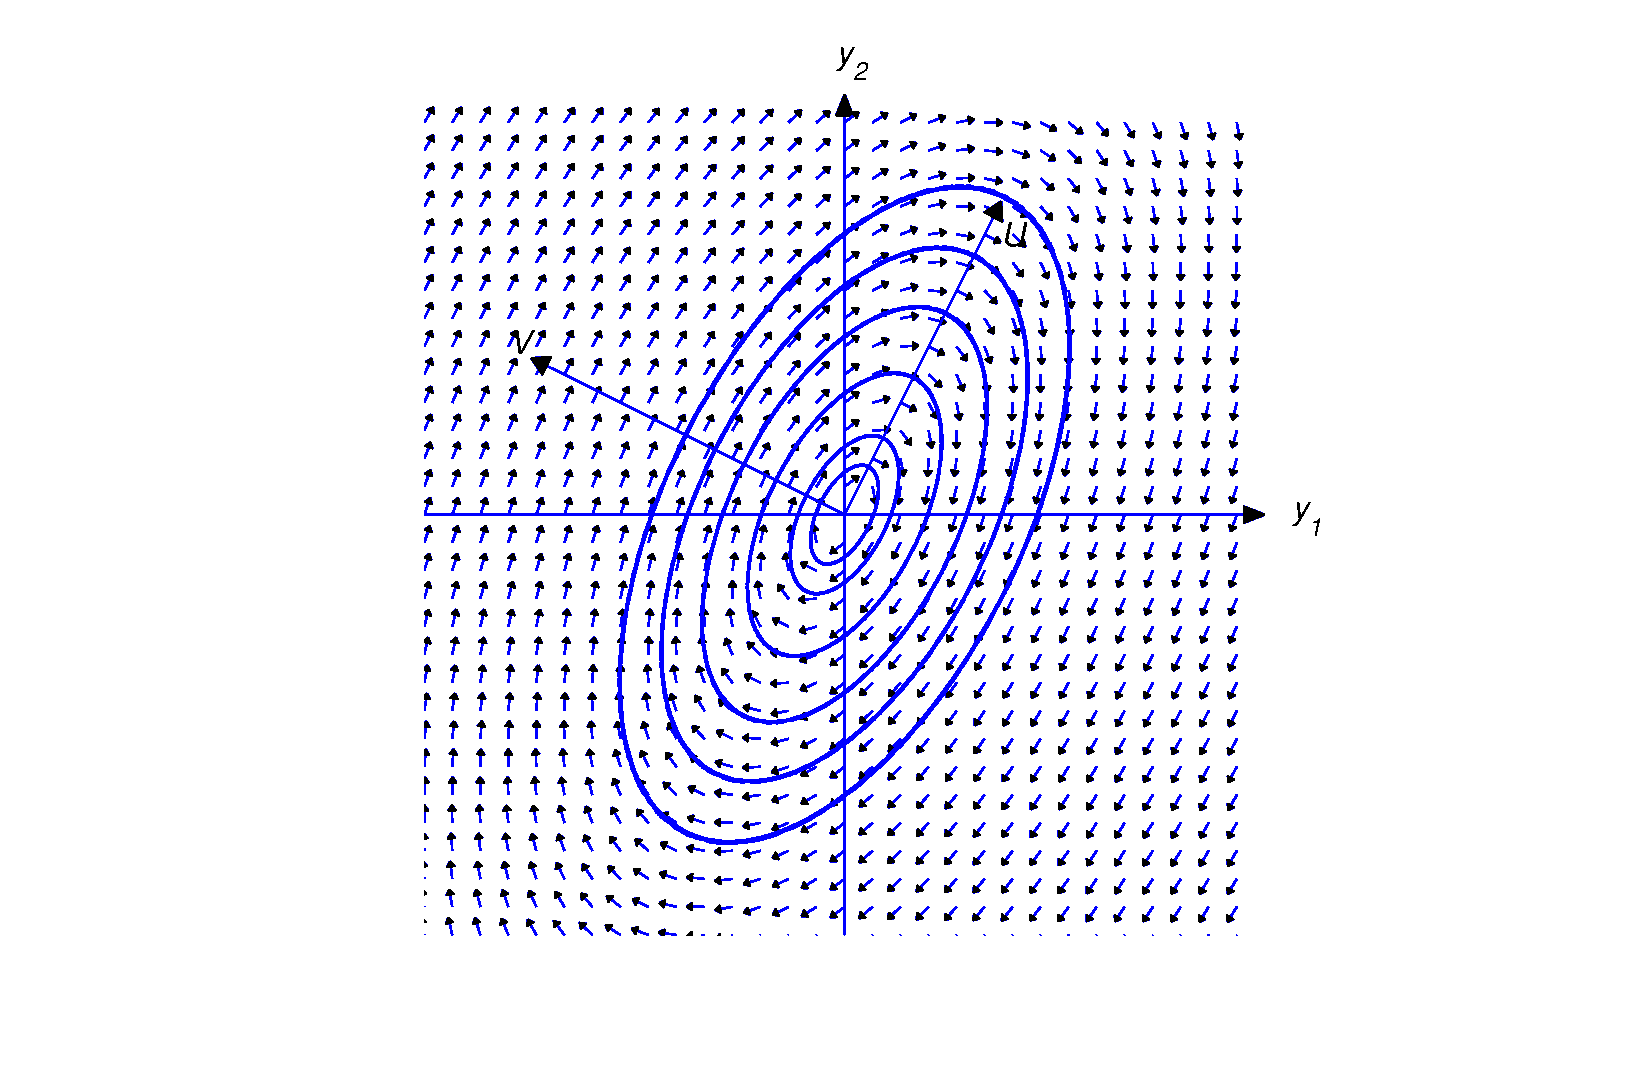
\includegraphics[bb=-78 148 689 643,width=5.67in,height=3.66in,keepaspectratio]{fig100601}}
\caption{ Shadow trajectories traversed clockwise}
  \label{figure:10.6.1}
\end{minipage}
  \begin{minipage}[b]{0.5\linewidth}
    \centering
   \scalebox{.65}{
  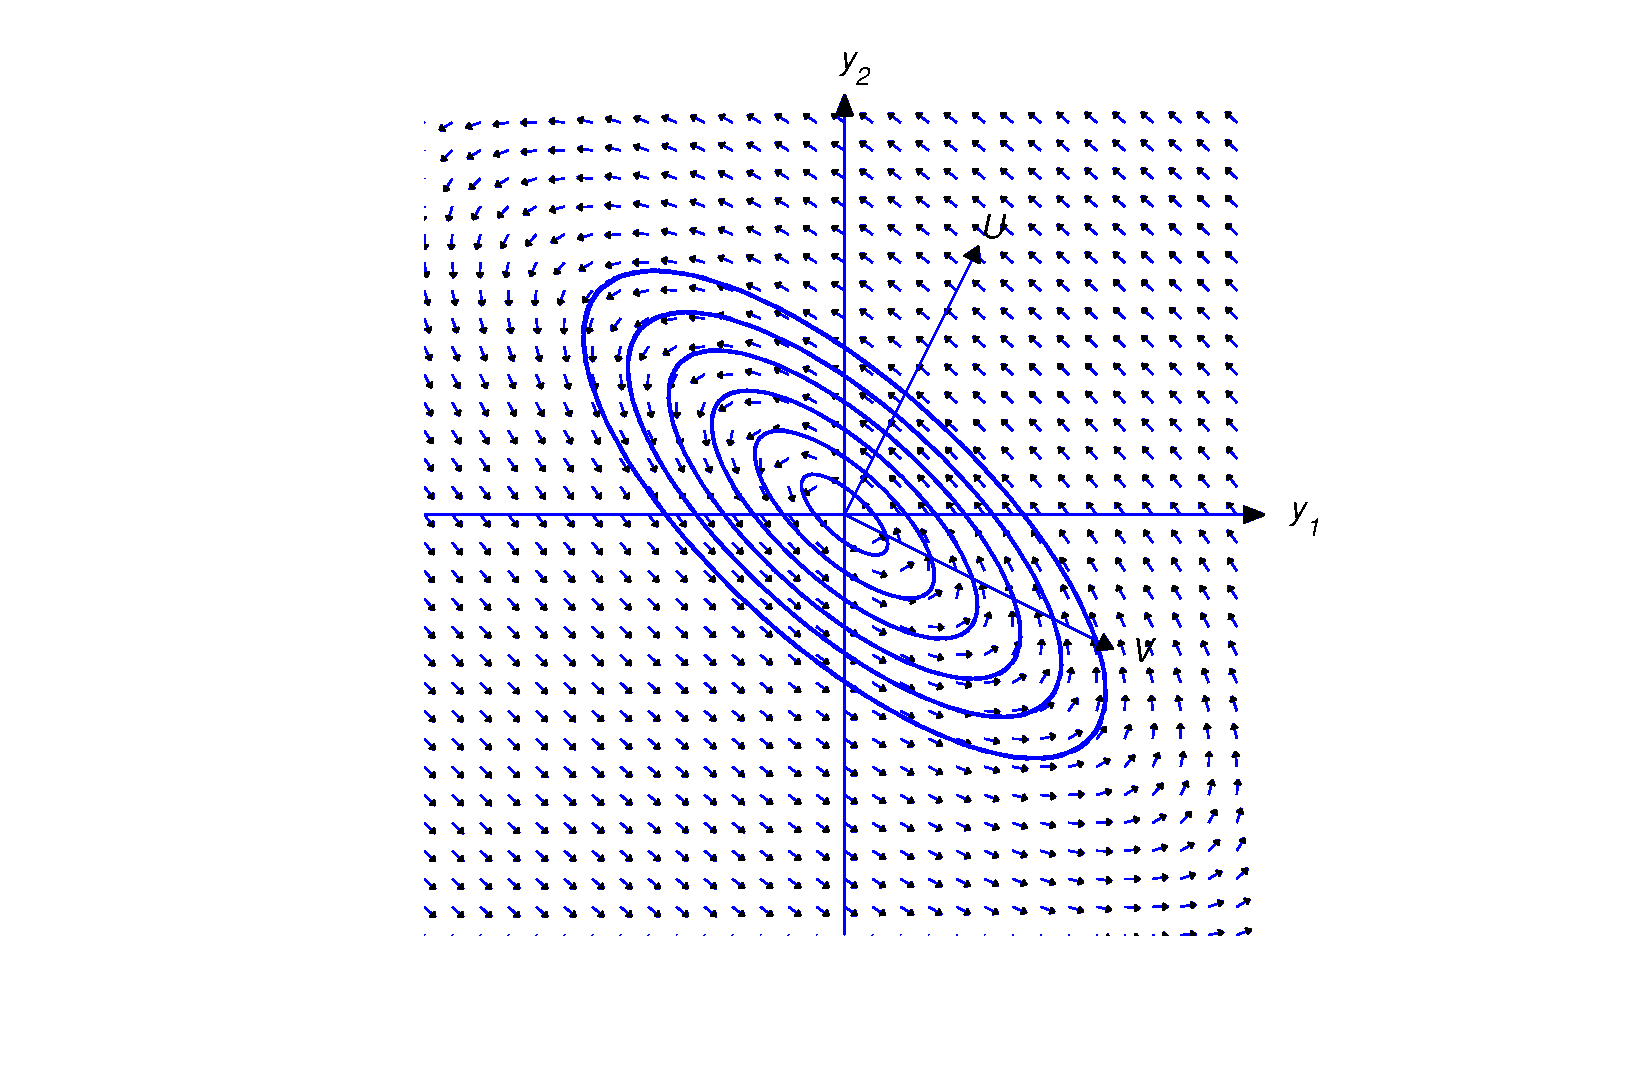
\includegraphics[bb=-78 148 689 643,width=5.67in,height=3.66in,keepaspectratio]{fig100602}}
\caption{ Shadow trajectories traversed counterclockwise}
  \label{figure:10.6.2}
\end{minipage}
\end{figure}

If $\alpha=0$, then any trajectory of \eqref{eq:10.6.10} is a shadow
trajectory of \eqref{eq:10.6.10};  therefore, if $\lambda$ is purely
imaginary, then the trajectories of \eqref{eq:10.6.10} are ellipses
traversed
periodically as indicated in Figures~\ref{figure:10.6.1} and
\ref{figure:10.6.2}.

If $\alpha>0$, then
$$
\lim_{t\to\infty}\|{\bf y}(t)\|=\infty\mbox{\quad and \quad}
\lim_{t\to-\infty}{\bf y}(t)=0,
$$
so the trajectory spirals away from the origin as $t$ varies from
$-\infty$ to $\infty$. The direction of the spiral depends upon the
relative orientation of ${\bf U}$ and ${\bf V}$, as shown in
Figures~\ref{figure:10.6.3} and \ref{figure:10.6.4}.

If $\alpha<0$,  then
$$
\lim_{t\to-\infty}\|{\bf y}(t)\|=\infty\mbox{\quad and \quad}
\lim_{t\to\infty}{\bf y}(t)=0,
$$
\enlargethispage{2in}
so the trajectory spirals toward the origin as $t$ varies from
$-\infty$ to $\infty$. Again, the direction of the spiral depends upon
the relative orientation of ${\bf U}$ and ${\bf V}$, as shown in
Figures~\ref{figure:10.6.5} and \ref{figure:10.6.6}.
\newpage

\begin{figure}[H]
\color{blue}
  \begin{minipage}[b]{0.5\linewidth}
    \centering
   \scalebox{.65}{
  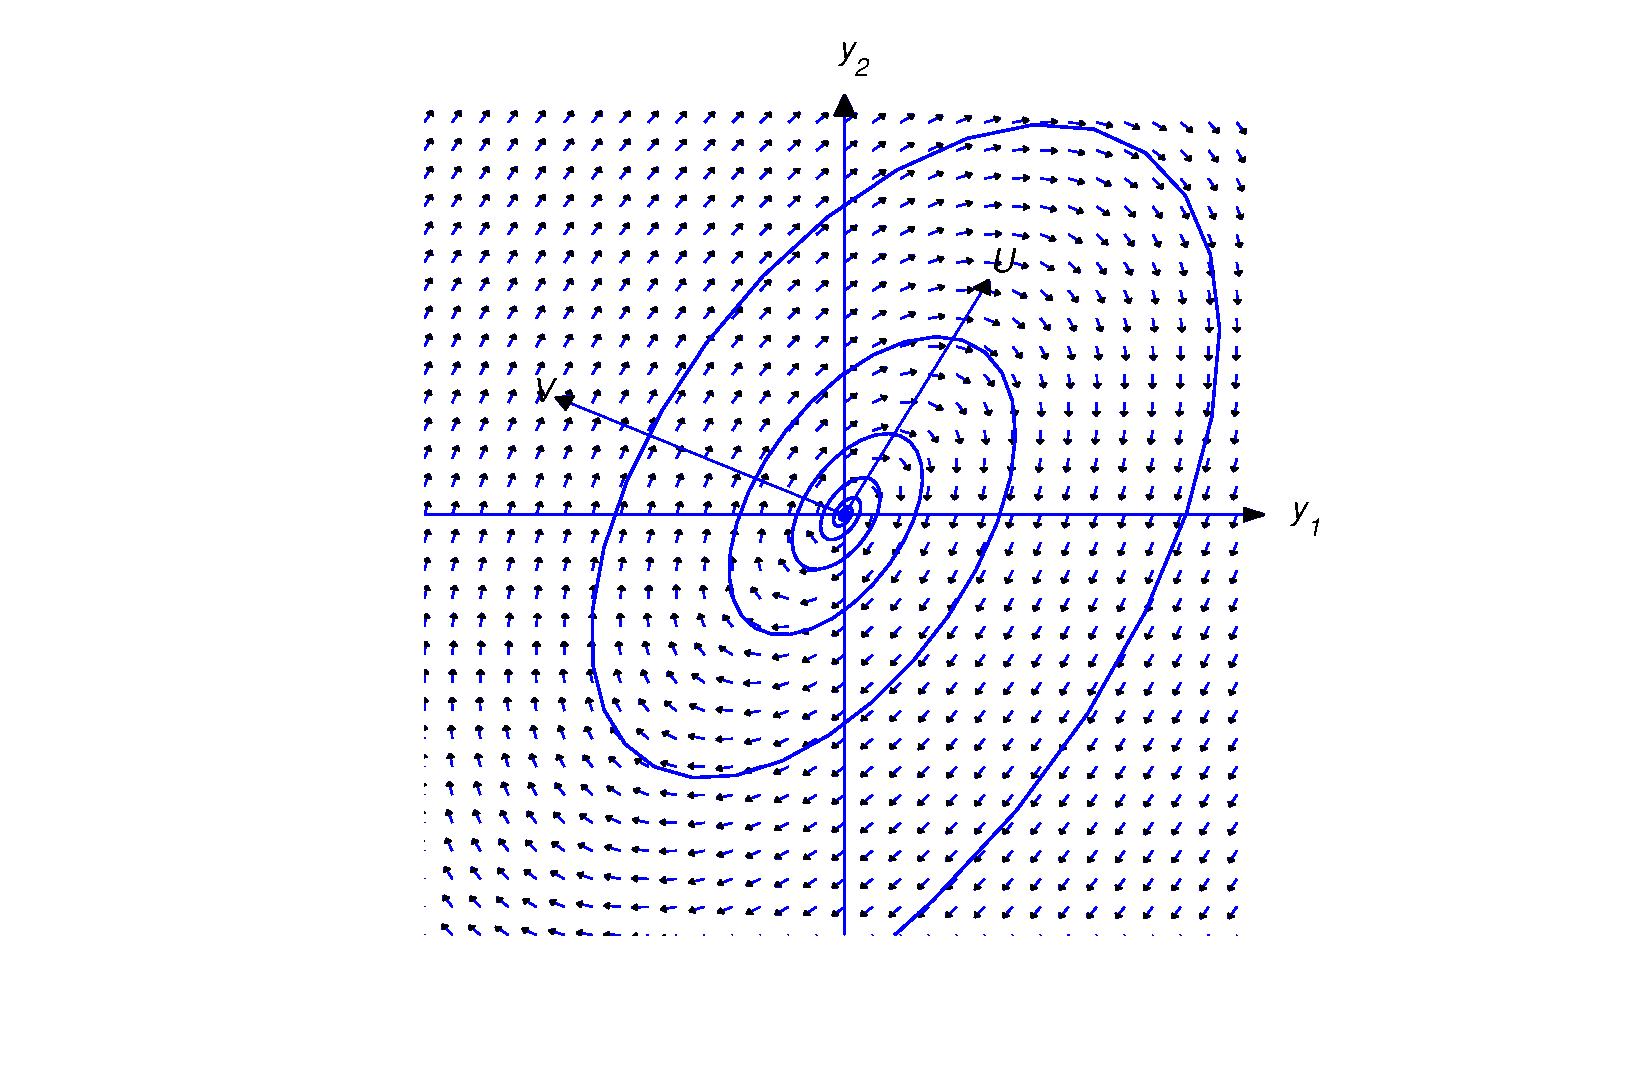
\includegraphics[bb=-78 148 689 643,width=5.67in,height=3.66in,keepaspectratio]{fig010603}}
\caption{ $\alpha>0$;   shadow trajectory spiraling outward}
  \label{figure:10.6.3}
\end{minipage}
  \begin{minipage}[b]{0.5\linewidth}
    \centering
   \scalebox{.65}{
  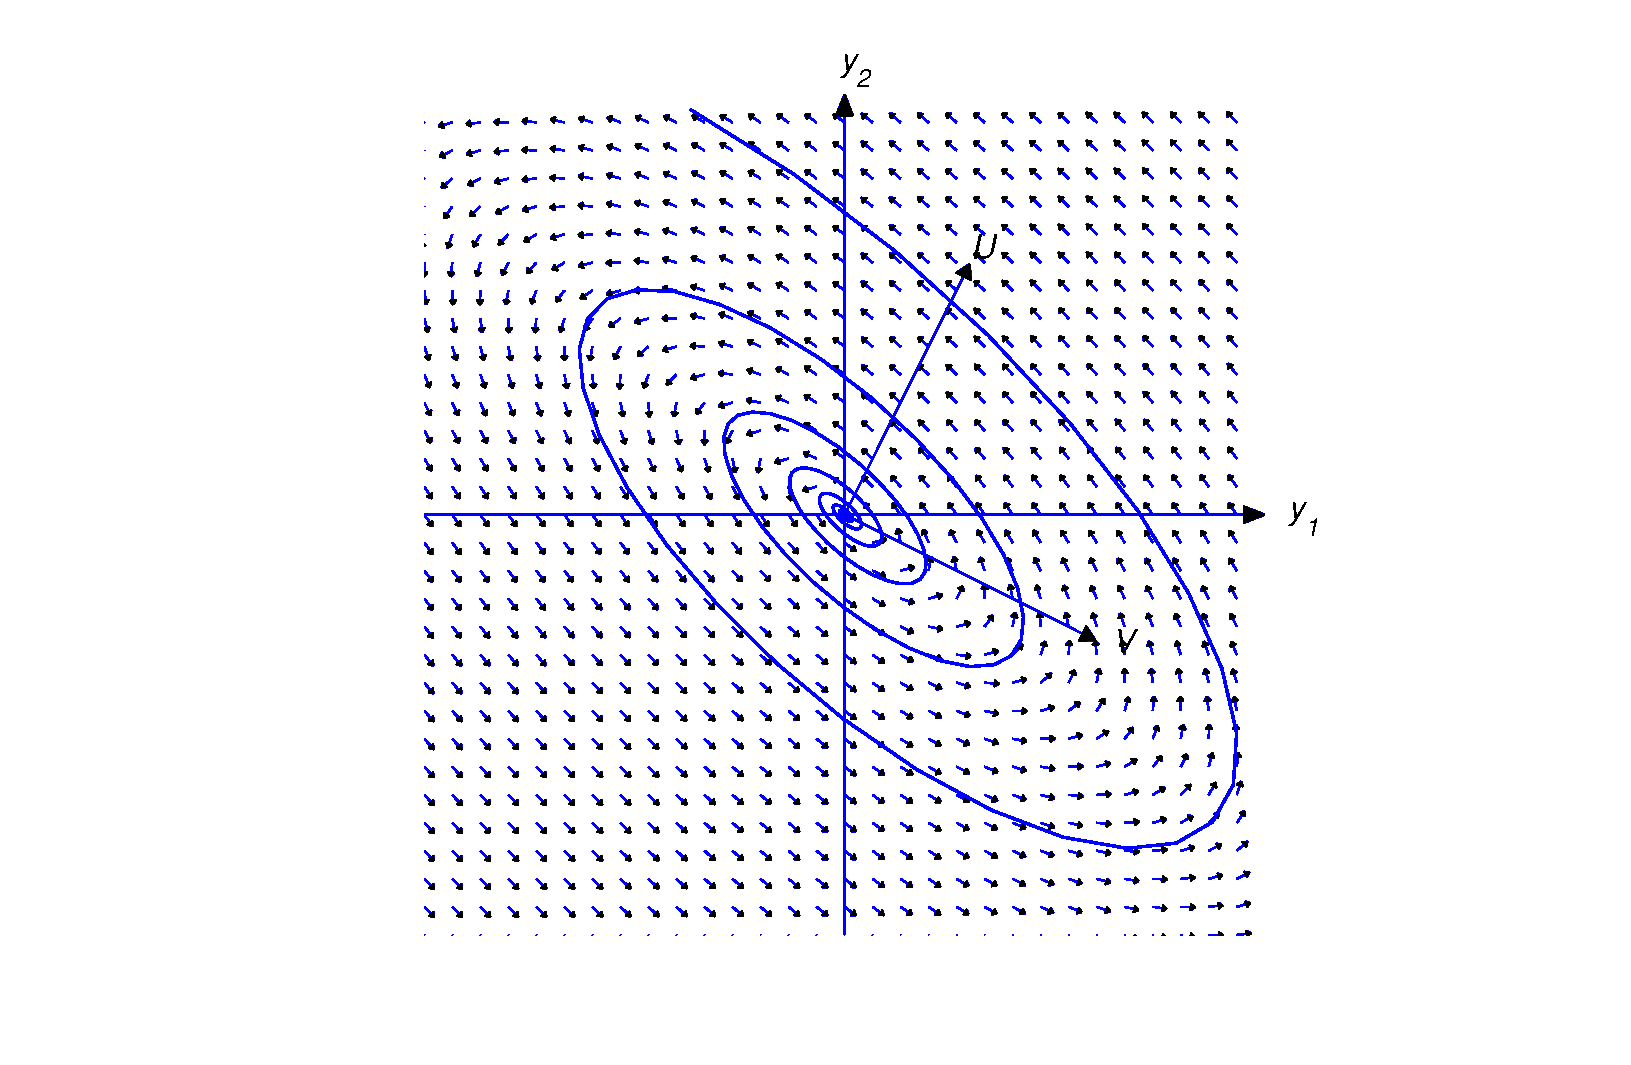
\includegraphics[bb=-78 148 689 643,width=5.67in,height=3.66in,keepaspectratio]{fig010604}}
\caption{ $\alpha>0$;   shadow trajectory spiraling outward}
  \label{figure:10.6.4}
\end{minipage}
\end{figure}

\begin{figure}[H]
\color{blue}
  \begin{minipage}[b]{0.5\linewidth}
    \centering
   \scalebox{.65}{
  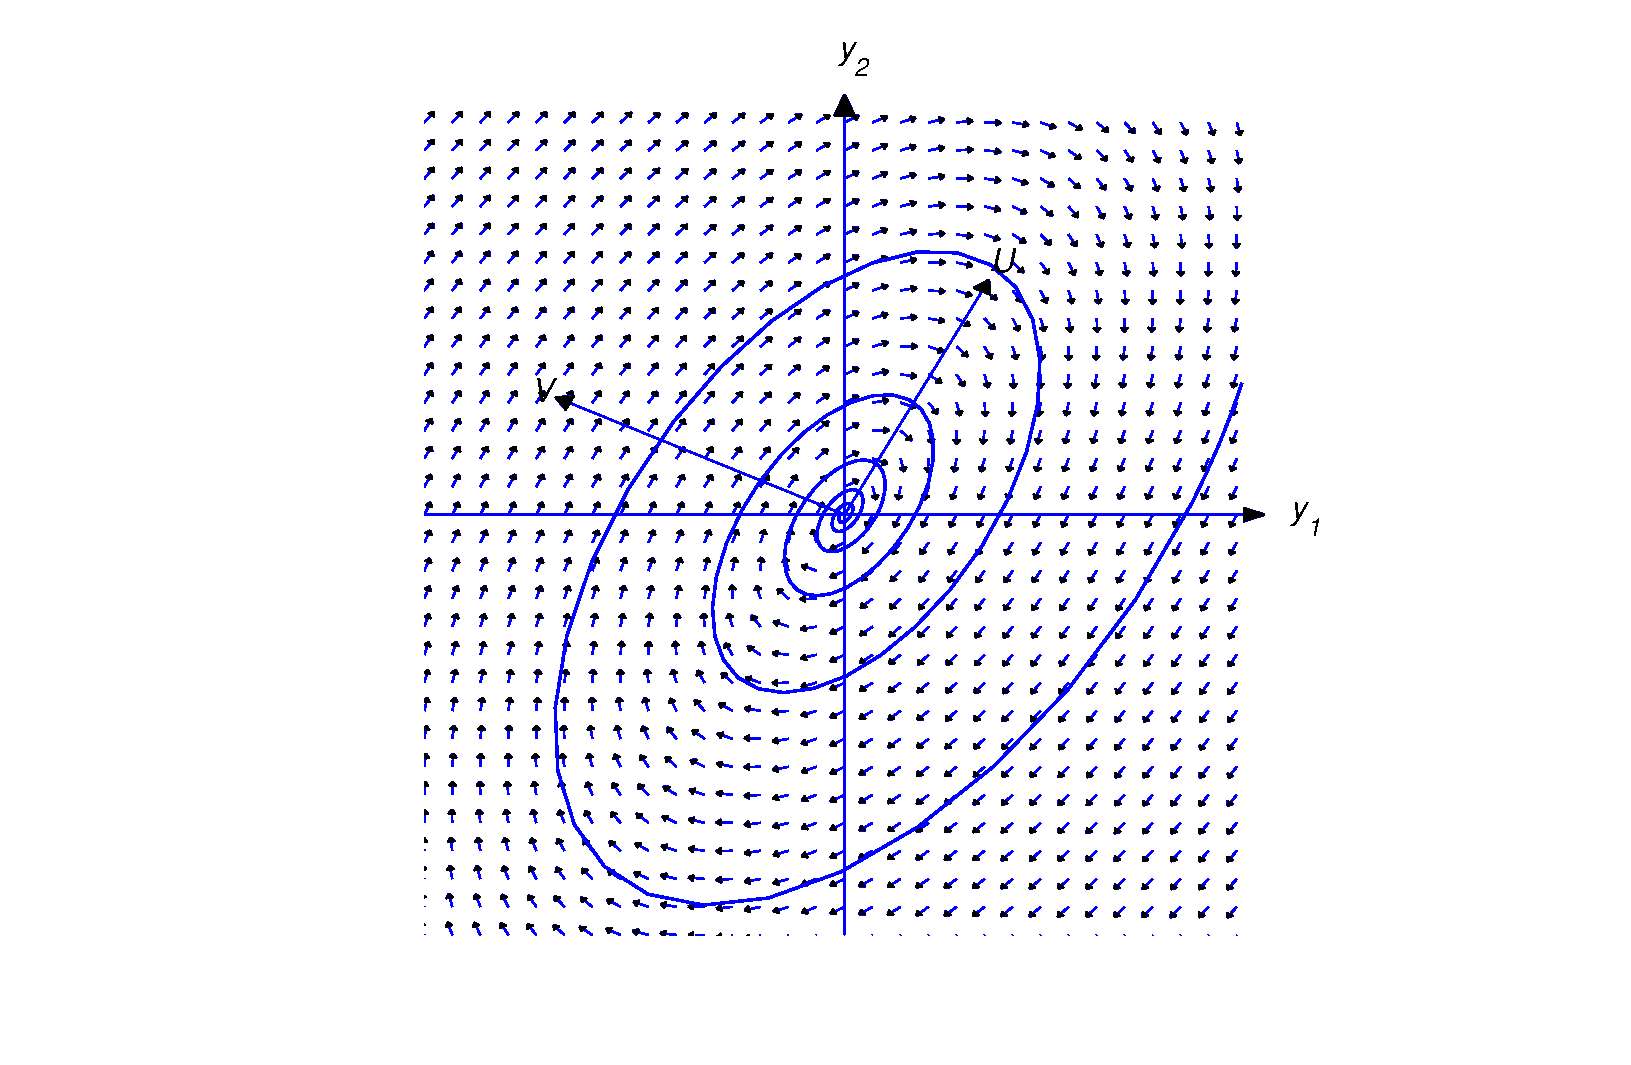
\includegraphics[bb=-78 148 689 643,width=5.67in,height=3.66in,keepaspectratio]{fig010605}}
\caption{ $\alpha<0$;   shadow trajectory spiraling inward}
  \label{figure:10.6.5}
\end{minipage}
  \begin{minipage}[b]{0.5\linewidth}
    \centering
   \scalebox{.65}{
  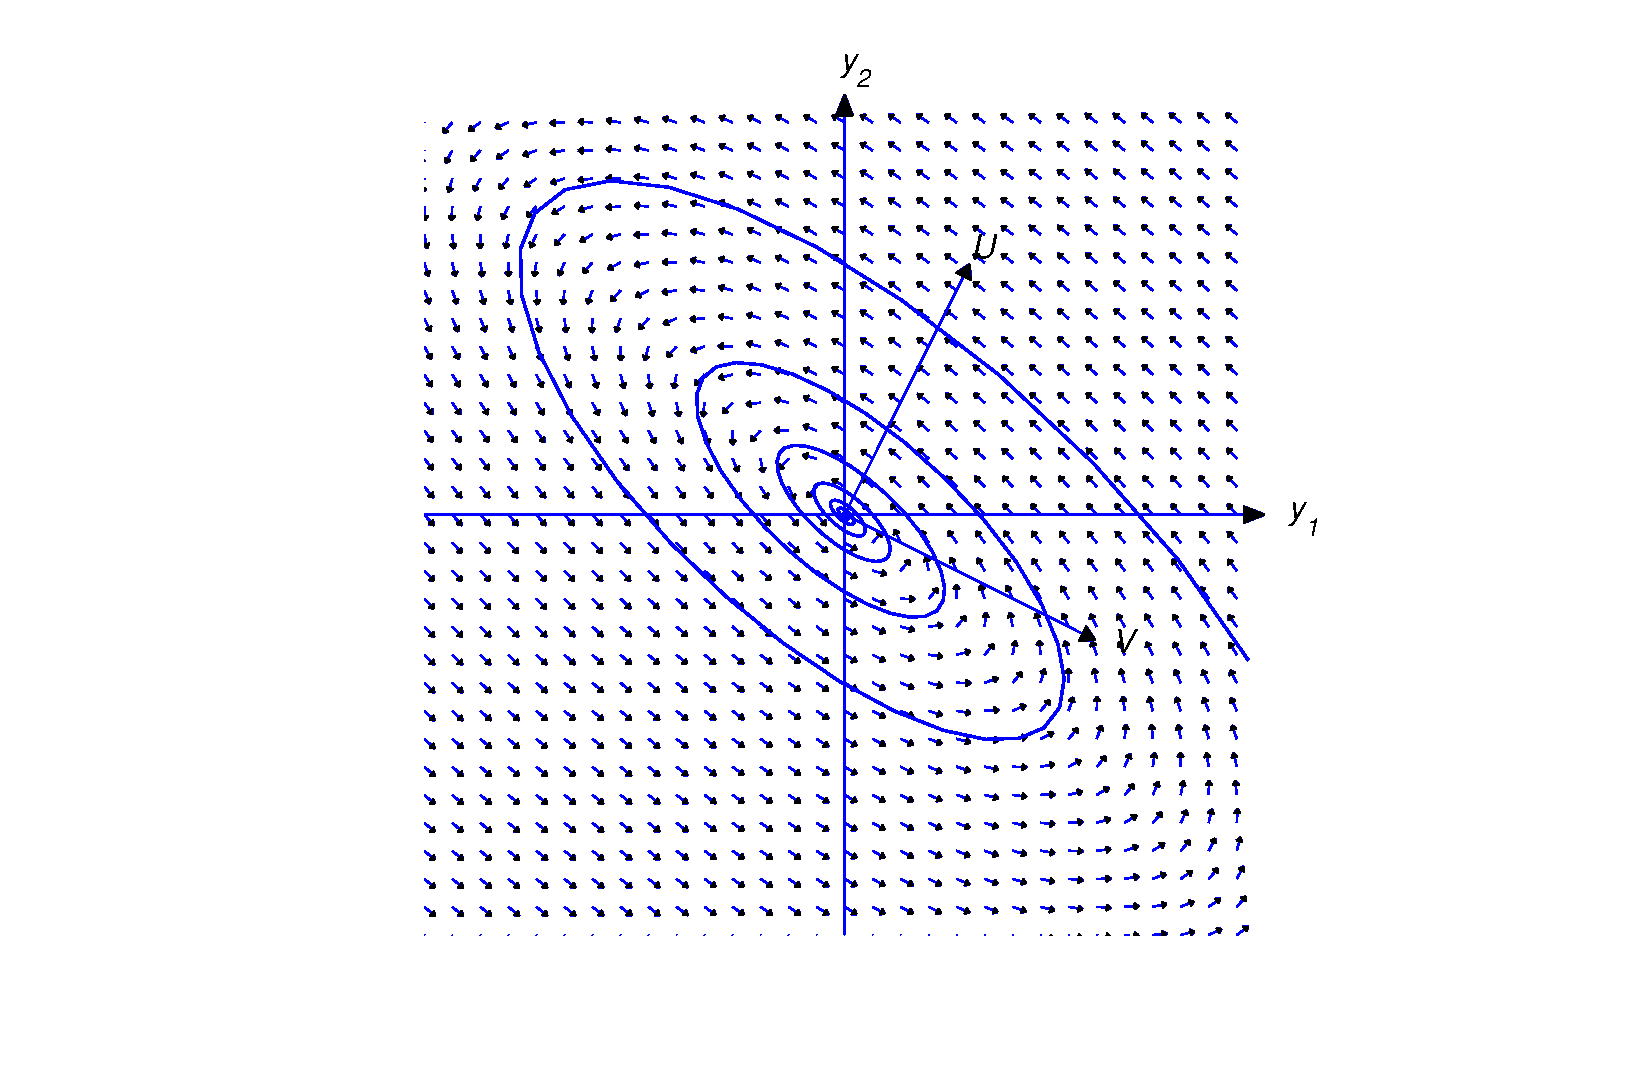
\includegraphics[bb=-78 148 689 643,width=5.67in,height=3.66in,keepaspectratio]{fig100606}}
\caption{ $\alpha<0$;   shadow trajectory spiraling inward}
  \label{figure:10.6.6}
\end{minipage}
\end{figure}

\exercises
In Exercises~\ref{exer:10.6.1}--\ref{exer:10.6.16}  find the general
solution.

\begin{exerciselist}
\begin{tabular}[t]{@{}p{168pt}@{}p{168pt}}
\item\label{exer:10.6.1}  $\dst{{\bf y}'=\twobytwo{-1}2{-5}5{\bf y}
}$&
\item\label{exer:10.6.2}  $\dst{{\bf y}'=\twobytwo{-11}4{-26}9{\bf y}
}$
\end{tabular}

\begin{tabular}[t]{@{}p{168pt}@{}p{168pt}}
\item\label{exer:10.6.3}  $\dst{{\bf y}'=\twobytwo12{-4}5{\bf y}}$&
\item\label{exer:10.6.4}  $\dst{{\bf y}'=\twobytwo5{-6}3{-1}{\bf y}}$
\end{tabular}

\begin{tabular}[t]{@{}p{168pt}@{}p{168pt}}
\item\label{exer:10.6.5}  $\dst{{\bf
y}'=\threebythree3{-3}1022511{\bf y}}$&
\item\label{exer:10.6.6}  $\dst{{\bf
y}'=\threebythree{-3}311{-5}{-3}{-3}73{\bf y}}$
\end{tabular}

\begin{tabular}[t]{@{}p{168pt}@{}p{168pt}}
\item\label{exer:10.6.7} $\dst{{\bf
y}'=\threebythree21{-1}011101{\bf y}}$&
\item\label{exer:10.6.8} $\dst{{\bf
y}'=\threebythree{-3}1{-3}4{-1}24{-2}3{\bf y}}$
\end{tabular}

\begin{tabular}[t]{@{}p{168pt}@{}p{168pt}}
\item\label{exer:10.6.9}  $\dst{{\bf y}'=\twobytwo5{-4}{10}1{\bf
y}}$&
 \item\label{exer:10.6.10}  $\dst{{\bf
y}'={1\over3}\twobytwo7{-5}25{\bf y}}$
\end{tabular}

\begin{tabular}[t]{@{}p{168pt}@{}p{168pt}}
\item\label{exer:10.6.11}  $\dst{{\bf y}'=\twobytwo32{-5}1{\bf y}}$&
\item\label{exer:10.6.12}  $\dst{{\bf
y}'=\twobytwo{34}{52}{-20}{-30}{\bf y}}$
\end{tabular}

\begin{tabular}[t]{@{}p{168pt}@{}p{168pt}}
\item\label{exer:10.6.13}  $\dst{{\bf y}'
=\threebythree11210{-1}{-1}{-2}{-1}{\bf y}}$&
\item\label{exer:10.6.14}  $\dst{{\bf y}'
=\threebythree3{-4}{-2}{-5}7{-8}{-10}{13}{-8}{\bf y}}$
\end{tabular}

\begin{tabular}[t]{@{}p{168pt}@{}p{168pt}}
\item\label{exer:10.6.15}  $\dst{{\bf
y}'=\threebythree60{-3}{-3}331{-2}6{\bf y}'}$&
\item\label{exer:10.6.16}  $\dst{{\bf
y}'=\threebythree12{-2}02{-1}100{\bf y}'}$
\end{tabular}

\exercisetext{In Exercises~\ref{exer:10.6.17}--\ref{exer:10.6.24}
solve the initial value problem.}

\item\label{exer:10.6.17}
$\dst{{\bf y}'=\twobytwo4{-6}3{-2}{\bf y},\quad {\bf
y}(0)=\twocol52}$

\item\label{exer:10.6.18}
$\dst{{\bf y}'=\twobytwo7{15}{-3}1{\bf y},\quad {\bf
y}(0)=\twocol51}$

\item\label{exer:10.6.19}
$\dst{{\bf y}'=\twobytwo7{-15}3{-5}{\bf y},\quad {\bf
y}(0)=\twocol{17}7}$

\item\label{exer:10.6.20}
$\dst{{\bf y}'={1\over6}\twobytwo4{-2}52{\bf y},\quad {\bf
y}(0)=\twocol1{-1}}$

\item\label{exer:10.6.21}
$\dst{{\bf y}'=\threebythree52{-1}{-3}22132{\bf y},\quad {\bf
y}(0)=\threecol406}$

\item\label{exer:10.6.22}
$\dst{{\bf y}'=\threebythree4408{10}{-20}23{-2}{\bf y},\quad {\bf
y}(0)=\threecol865}$

\item\label{exer:10.6.23}
$\dst{{\bf
y}'=\threebythree1{15}{-15}{-6}{18}{-22}{-3}{11}{-15}{\bf
y},\quad {\bf y}(0)=\threecol{15}{17}{10}}$

\item\label{exer:10.6.24}
$\dst{{\bf y}'=\threebythree4{-4}4{-10}3{15}2{-3}1{\bf y},\quad
{\bf y}(0)=\threecol{16}{14}6}$

\item\label{exer:10.6.25}
Suppose an $n\times n$ matrix $A$ with
real entries has a complex eigenvalue $\lambda=\alpha+i\beta$
($\beta\ne0$) with associated eigenvector ${\bf x}={\bf u}+i{\bf v}$,
where ${\bf u}$ and ${\bf v}$ have real components. Show that ${\bf
u}$ and ${\bf v}$ are both nonzero.

\item\label{exer:10.6.26}
Verify that
$$
{\bf y}_1=e^{\alpha t}({\bf u}\cos\beta t-{\bf v}\sin\beta t)
\mbox{\quad and\quad}
{\bf y}_2=e^{\alpha t}({\bf u}\sin\beta t+{\bf v}\cos\beta t),
$$
are the real and imaginary parts of
$$
e^{\alpha t}(\cos\beta t+i\sin\beta t)({\bf u}+i{\bf v}).
$$

\item\label{exer:10.6.27}
 Show that if the vectors ${\bf u}$ and ${\bf v}$ are not both ${\bf
0}$ and $\beta\ne0$ then the vector functions
$$
{\bf y}_1=e^{\alpha t}({\bf u}\cos\beta t-{\bf v}\sin\beta t)\quad
\mbox{ and }\quad
{\bf y}_2=e^{\alpha t}({\bf u}\sin\beta t+{\bf v}\cos\beta t)
$$
are linearly independent on every interval. \hint{There are
two
cases to consider: {\rm(i)} $\{{\bf u},{\bf v}\}$ linearly
independent, and {\rm(ii)}
 $\{{\bf u},{\bf v}\}$ linearly dependent. In either case, exploit the linear independence of $\{\cos\beta t,\sin\beta t\}$
on every interval.}

\item\label{exer:10.6.28}
Suppose ${\bf u}=\dst{\twocol{u_1}{u_2}}$ and ${\bf
v}=\dst{\twocol{v_1}{v_2}}$ are not orthogonal; that is, $({\bf
u},{\bf v})\ne0$.
\begin{alist}
\item % (a)
Show that  the quadratic equation
$$
({\bf u},{\bf v})k^2+(\|{\bf v}\|^2-\|{\bf u}\|^2)k-({\bf u},{\bf
v})=0
$$
has a positive root $k_1$ and a negative root $k_2=-1/k_1$.
\item % (b)
Let ${\bf u}_1^{(1)}={\bf u}-k_1{\bf v}$, ${\bf v}_1^{(1)}={\bf
v}+k_1{\bf u}$, ${\bf u}_1^{(2)}={\bf u}-k_2{\bf v}$, and ${\bf
v}_1^{(2)}={\bf v}+k_2{\bf u}$, so that $({\bf u}_1^{(1)},{\bf
v}_1^{(1)}) =({\bf u}_1^{(2)},{\bf v}_1^{(2)})=0$, from the discussion
given above. Show that
$$
{\bf u}_1^{(2)}={{\bf v}_1^{(1)}\over k_1}
\mbox{\quad and \quad}
{\bf v}_1^{(2)}=-{{\bf u}_1^{(1)}\over k_1}.
$$
\item % (c)
Let ${\bf U}_1$, ${\bf V}_1$, ${\bf U}_2$, and ${\bf V}_2$ be unit
vectors in the directions of ${\bf u}_1^{(1)}$, ${\bf v}_1^{(1)}$,
${\bf u}_1^{(2)}$, and ${\bf v}_1^{(2)}$, respectively. Conclude from
\part{a} that ${\bf U}_2={\bf V}_1$ and ${\bf V}_2=-{\bf U}_1$, and
that therefore the counterclockwise angles from ${\bf U}_1$ to ${\bf
V}_1$ and from ${\bf U}_2$ to ${\bf V}_2$ are both $\pi/2$ or both
$-\pi/2$.
\end{alist}

\exercisetext{In Exercises~\ref{exer:10.6.29}-\ref{exer:10.6.32} find vectors
${\bf U}$ and ${\bf V}$ parallel to the axes of symmetry of the
trajectories, and plot some typical trajectories.}

\begin{tabular}[t]{@{}p{168pt}@{}p{168pt}}
\item\label{exer:10.6.29} \CGex\, $\dst{{\bf y}'=\twobytwo3{-5}5{-3}{\bf
y}}$&
\item\label{exer:10.6.30} \CGex\,  $\dst{{\bf y}'=\twobytwo{-15}{10}{-25}{15}{\bf y}}$
\end{tabular}

\begin{tabular}[t]{@{}p{168pt}@{}p{168pt}}
\item\label{exer:10.6.31} \CGex\,  $\dst{{\bf y}'=\twobytwo{-4}8{-4}4{\bf y}}$&
\item\label{exer:10.6.32} \CGex\,  $\dst{{\bf y}'=\twobytwo{-3}{-15}33{\bf y}}$
\end{tabular}

\exercisetext{In Exercises~\ref{exer:10.6.33}-\ref{exer:10.6.40} find vectors
${\bf U}$ and ${\bf V}$ parallel to the axes of symmetry of the shadow
trajectories, and plot a typical trajectory.}

\begin{tabular}[t]{@{}p{168pt}@{}p{168pt}}
\item\label{exer:10.6.33} \CGex\,  $\dst{{\bf y}'=\twobytwo{-5}6{-12}7{\bf y}}$&
\item\label{exer:10.6.34} \CGex\,  $\dst{{\bf y}'=\twobytwo5{-12}6{-7}{\bf y}}$
\end{tabular}

\begin{tabular}[t]{@{}p{168pt}@{}p{168pt}}
\item\label{exer:10.6.35} \CGex\,  $\dst{{\bf y}'=\twobytwo4{-5}9{-2}{\bf y}}$&
\item\label{exer:10.6.36} \CGex\,  $\dst{{\bf y}'=\twobytwo{-4}9{-5}2{\bf y}}$
\end{tabular}

\begin{tabular}[t]{@{}p{168pt}@{}p{168pt}}
\item\label{exer:10.6.37} \CGex\,  $\dst{{\bf y}'=\twobytwo{-1}{10}{-10}{-1}{\bf y}}$&
\item\label{exer:10.6.38} \CGex\,  $\dst{{\bf y}'=\twobytwo{-1}{-5}{20}{-1}{\bf y}}$
\end{tabular}

\enlargethispage{1in}
\begin{tabular}[t]{@{}p{168pt}@{}p{168pt}}
\item\label{exer:10.6.39} \CGex\,  $\dst{{\bf y}'=\twobytwo{-7}{10}{-10}9{\bf y}}$&
\item\label{exer:10.6.40} \CGex\,  $\dst{{\bf y}'=\twobytwo{-7}6{-12}5{\bf y}}$
\end{tabular}

\end{exerciselist}
